\documentclass[11pt, a4paper]{article}
\usepackage{opgave}
\usepackage{fancyStyle}
\usepackage{hyperref}
\usepackage{listings}

\renewcommand{\course}{DEV01-1}
\renewcommand{\titel}{Assignment 5}
\renewcommand{\auteur}{The INFDEV Team @ HR}
\renewcommand{\auteurlang}{\auteur}

\setboolean{isTentamen}{false}
\setboolean{showAntwoord}{false}

\usepackage{graphicx}

\begin{document}
\setcounter{opgave}{1}
This is the second of the three assignments that will be graded.
You can score a maximum of $3$ points for this assignment, 1 point for each exercise.

\opgave{Reverse}{1}
\subopgave{Write a program that asks for a user’s input and prints that string in reverse.
}{}{1}
Example input -> output
\begin{itemize}
\item “Beautiful is better than ugly.” -> “.ylgu naht retteb si lufituaeB”
\end{itemize}


\opgave{Passwords}{1}
 \subopgave{Write a program that calculates how secure a password is (weak, medium, strong). You can come up with your own calculation, but at least take into account: the amount of characters and the diversity of characters (lowercase, uppercase, numbers and special characters).
  }{}{0}

  \begin{itemize}
   \item the password ''a'' is weak
   \item the password ''Tr0ub4dor\&3'' is medium
   \item the password ''correct horse battery staple'' is strong\footnote{Mandatory nerdy comic: \url{https://xkcd.com/936/}}
  \end{itemize}

\opgave{Cryptography}{1}
 \subopgave{
 Write a program that asks the user for an input string and a number n.
 The program should output that string, but with every letter shifted with the amount of n.
 For example ‘B’ shifted by 3 would become ‘E’.

 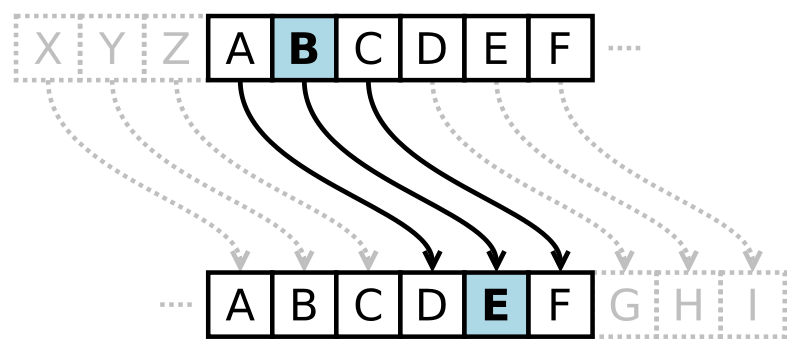
\includegraphics[width=6cm]{crypto.png}
 }{}{0}

example input → output:
 \begin{itemize}
 \item ''a'', 1 -> ''b''
 \item ''ab c'', 1 -> ''bc d''
 \item ''aBc'', 2 ->''cDe''
 \item ''xyz?'', -20 -> ''def?''
 \item ''z'', 1 -> ''a''
 \end{itemize}

 \begin{itemize}
\item You may use the ord()-function to convert a character to its ascii integer value
\item You may use the input (or raw\_input) function twice, once for the string and once for the number n
\item A capital letter in the input should result in a capital letter in the output, the same holds for lower case letters
\item Non-letter characters should remain untouched
 \end{itemize}

\einde
\end{document}